%
%  Thesis main document
%
%  Created by Mathias Dalheimer on 2007-02-14
%  Copyright (c) 2007. All rights reserved.
%
\documentclass[11pt]{article}

% Use utf-8 encoding for foreign characters
\usepackage[utf8]{inputenc}

% Setup for fullpage use
\usepackage{fullpage}
\usepackage{url}
%\usepackage{german}

% Uncomment some of the following if you use the features
%
% Running Headers and footers
%\usepackage{fancyhdr}
%\pagestyle{fancy} % options: empty , plain , fancy
%\renewcommand{\headrulewidth}{1pt} % customise the layout...
%\lhead{}\chead{}\rhead{}
%\lfoot{}\cfoot{\thepage}\rfoot{}

%\fancyhead[LE,RO]{\slshape \rightmark} 
%\fancyhead[LO,RE]{\slshape \leftmark} 
%\fancyfoot[LE, RO]{\thepage} 

%%% SECTION TITLE APPEARANCE
\usepackage{sectsty}
\allsectionsfont{\sffamily\mdseries\upshape} % (See the fntguide.pdf for font help)
% (This matches ConTeXt defaults)

\setlength{\parindent}{0cm}
\clubpenalty=1500
\widowpenalty=2000

\usepackage{ngerman}

% Multipart figures
%\usepackage{subfigure}
%\usepackage{lib/algorithm2e}

% More symbols
\usepackage{amsmath}
%\usepackage{amssymb}
\usepackage{latexsym}

% Surround parts of graphics with box
%\usepackage{boxedminipage}

% Package for including code in the document
%\usepackage{listings}

% If you want to generate a toc for each chapter (use with book)
%\usepackage{minitoc}

% This is now the recommended way for checking for PDFLaTeX:
\usepackage{ifpdf}

%\newif\ifpdf
%\ifx\pdfoutput\undefined
%\pdffalse % we are not running PDFLaTeX
%\else
%\pdfoutput=1 % we are running PDFLaTeX
%\pdftrue
%\fi

\ifpdf
\usepackage[pdftex]{graphicx}
\else
\usepackage{graphicx}
\fi


\usepackage{listings}  
\lstset{numbers=left, numberstyle=\tiny,numbersep=5pt}  
\lstset{language=Xml, basicstyle=\small, frame=shadowbox}  

\usepackage[hypertexnames=false,pdftex]{hyperref}
\hypersetup{
pdfauthor = {Mathias Dalheimer},
pdftitle = {Designing Message-oriented Applications with MQS and
SEDA}
pdfsubject = {},
pdfkeywords = {Grid Computing}
pdfcreator = {LaTeX with hyperref package},
pdfproducer = {dvips + ps2pdf}}
\usepackage{algorithmic}
\usepackage{algorithm}
\renewcommand{\algorithmicrequire}{\textbf{Input:}} 
\renewcommand{\algorithmicensure}{\textbf{Output:}}

%%%%%%%%%%%%%%%%%%%%%%%%%%%%%%%%%%%%%%%%%%%%%%%%%%%%%%%%%%%%%%%%%%%%
\newcommand{\outcome}[1]{\mathtt{#1}}
\newcommand{\jobpredicate}[1]{\mathtt{#1}}

\newcommand{\stateset}{\mathcal{S}}
\newcommand{\actionset}{\mathcal{A}}
\newcommand{\transprob}{\mathcal{P}}
\newcommand{\reward}{\mathcal{R}}
\newcommand{\return}{\mathit{R}}
\newcommand{\policy}{\pi}
\newcommand{\plainstatevaluefunct}[1]{V^{#1}}
\newcommand{\statevaluefunct}{\plainstatevaluefunct{\policy}}
\newcommand{\optstatevaluefunct}{\plainstatevaluefunct{*}}
\newcommand{\actionvaluefunct}{Q^\policy}
\newcommand{\optactionvaluefunct}{Q^*}
%%%%%%%%%%%%%%%%%%%%%%%%%%%%%%%%%%%%%%%%%%%%%%%%%%%%%%%%%%%%%%%%%%%%
\newcommand{\PG}{PHASTGrid\ }
\newcommand{\SM}{Storagemanager\ }

\title{\textsf{Designing Message-oriented Applications with libmqs and
libseda}}
\author{ Mathias Dalheimer\\
\url{dalheimer@itwm.fhg.de}}

\date{Version 0.1, \today\\
}

\begin{document}

\ifpdf
\DeclareGraphicsExtensions{.pdf, .jpg, .tif}
\else
\DeclareGraphicsExtensions{.eps, .jpg}
\fi

\maketitle


\tableofcontents

\section{Introduction}\label{sec:introduction}
Building  blocks  of message-oriented  applications  are message  brokers.
Clients  connect to  message  brokers and  exchange  messages adressed  to
logocal URIs instead  of communicating directly with each  other. In order
to support  the development  of message-oriented applications,  the libmqs
and libseda libraries have been written.

\section{The SEDA library}\label{sec:libseda}
The \verb|libseda|  is an implemenation  of the \emph{Staged  Event Driven
  Architecture} (SEDA) architectural approach \cite{seda-approach} written
in C++.  An application is split up into several independent \emph{stages}
which communicate with each other using events.  Each stage consists of an
incoming  event-queue  and  a   thread  pool.   The  stage's  threads  are
responsible for performing the special  task of the stage --- they consume
messages from the incoming queue and  generate new events that are sent to
other stages of the application.

\subsection{Building blocks}
\label{sec:libseda:building-blocks}

The  library  contains several  classes  that  are  crucial for  the  SEDA
approach.   These  classes  are:  \verb|Stage|,  \verb|StageRegistry|  and
\verb|Strategy|.  As  stated before,  a stage is  represented by  a thread
pool and  an incoming event  queue. The work  that the threads of  a stage
perform is defined by an implementation of the Strategy interface. Thus, a
stage contains  a Strategy, too. The StageRegistry  contains mappings from
the name  of a stage to  the stage itself  (each stage must have  a unique
name when  it is created)  --- the purpose  of this class is  to eliminate
cyclic dependencies when building up an application. The simplest included
Strategy that uses the StageRegistry  is the ForwardStrategy.  As the name
suggests, this strategy simply forwards any event to another stage.

\subsection{Supportive classes}\label{sec:libseda:supportiveclasses}
The  concept of  splitting up  a  stage into  a generic  part ---  message
handling and encapsulation of the  thread pool --- and the actual behavior
part   follows   the   well-known  Strategy   pattern   (\cite{gof-book}).
Furthermore  Strategies  can  build  up  a Strategy  hierarchy  using  the
Decorator pattern. For example, if one  likes to add logging output to the
events  handled by  a particular  stage, he  simply augments  the existing
strategy of that stage with a LoggingStrategy. This means before the event
is handled by the old strategy it gets logged.

The EventCountStrategy is  most useful when performing unit  tests of your
application. One simply  enhances a stage's strategy to  count all handled
events. After running  the test case, simply check  if the expected number
of events have been seen by that stage.

A code snippet that shows how a strategy decorates another looks like:
\begin{verbatim}
seda::Strategy::Ptr fwd(new seda::ForwardStrategy("next stage"));
fwd = seda::Strategy::Ptr(new seda::LoggingStrategy(fwd));
seda::Stage::Ptr s(new seda::Stage("first stage", fwd));
\end{verbatim}


\section{Anatomy of an Application}\label{sec:anatomy of an application}
As a quick  introduction, I will present some of  the functionality of the
libraries  in  this  section.  I  assume you're  familiar  with  the  SEDA
architectural approach. Basically,  applications process incoming messages
in stages.  Each stage  contains a threadpool.  Stages are  separated with
queues. The  work to be done  is put in the  inqueue of a  stage. A thread
dequeues it and applies a strategy to it. Depending on the strategy one or
several messages  are issued to the  environment - which  means that other
stages  might pick  them  up.  Decorators provide  another  way of  adding
behaviour to a stage: Think of them  as a FIFO pipe that all messages must
pass before they are processed.

The libmqs provides abstractions for connecting to a message broker,
sending and receiving messages etc.
\begin{figure}[htbp]
  \begin{center}
    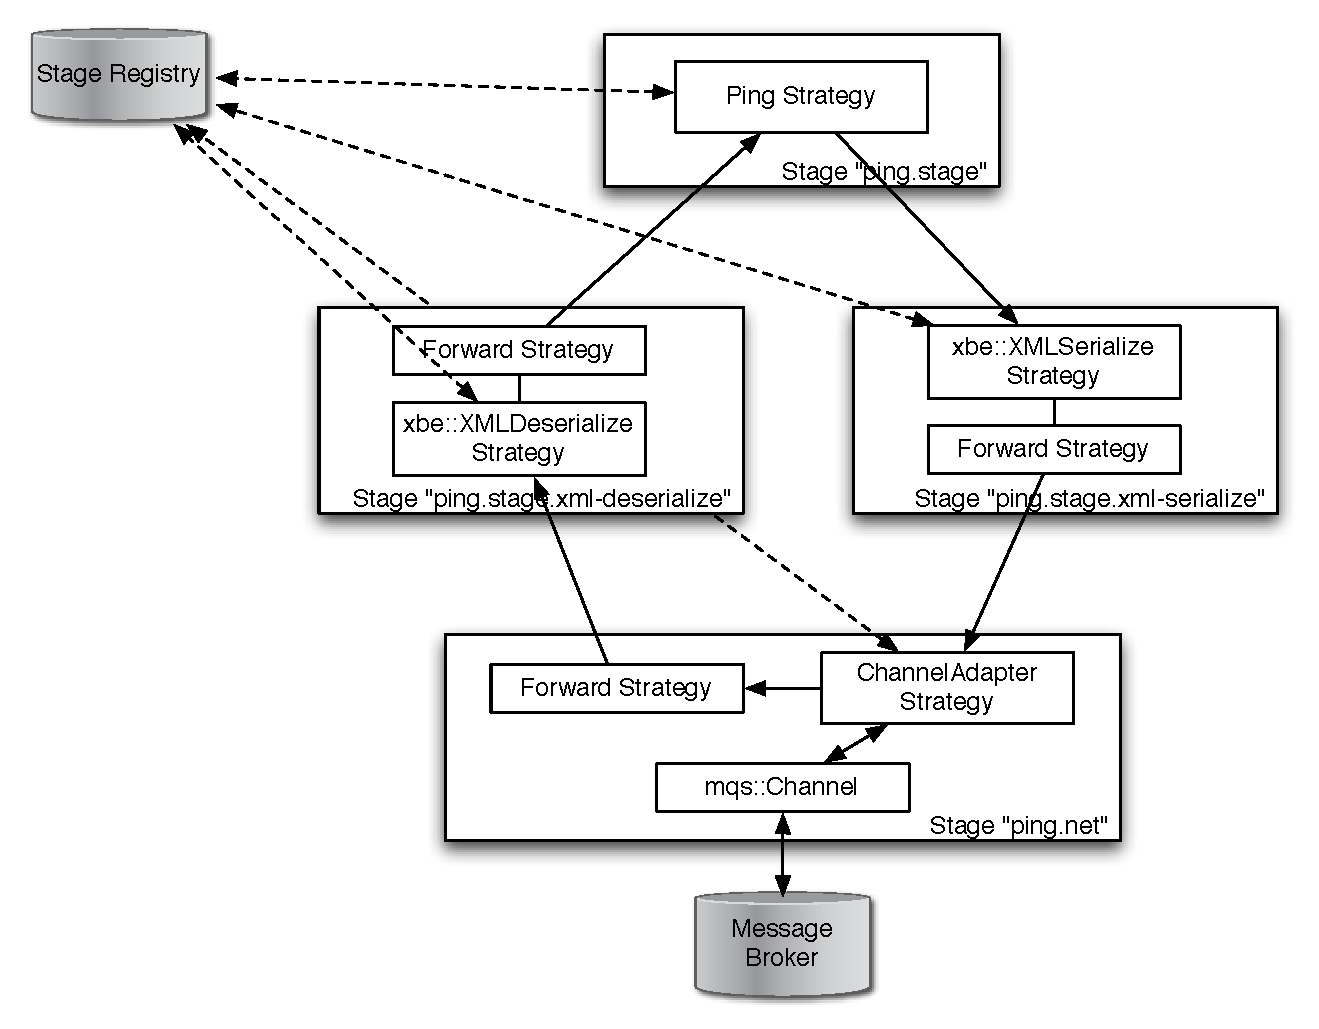
\includegraphics[width=12cm]{MQS-SEDA-Architecture.pdf}
    \caption{The building blocks of the Pingpong architecture. Only
    the Ping part is shown.}
    \label{fig:mqs-seda-architecture}
  \end{center}
\end{figure}

The easiest way to understand this is to look at some application. I
use the famous PingPong example where two application send each other
"`ping"' and "`pong"' messages. You can find the corresponding source
code in \verb|xbe/tests/xbe/PingPongTest.cpp|. 

The    structure    of    the    application   is    shown    in    figure
\ref{fig:mqs-seda-architecture}. The  connection to the  Message Broker is
made  in  the "`ping.net"'  stage.  An  mqs  Channel object  receives  the
messages and  puts them in  the ChannelAdapter Strategy inqueue.  They are
then  forwarded to  the xml-deserialize  stage, where  an XML  encoding is
removed. Again, the  messages are forwarded to the  "`ping.stage"' where a
Ping  Strategy implements  the behaviour  of  the application  - i.e.,  it
responds  with a  "`pong"'  message for  each  incoming "`ping"'  message.
Outgoing  messages  are serialized  and  forwarded  to the  ChannelAdapter
strategy, which sends them over the mqs Channel to the Message Broker.

The connection between the different stages is made through the Stage
Registry. At startup, all stages register themselves with a unique
identifier at the registry. The ForwardStrategies (and the PingStrategy)
are initialized with the identifier of the Strategy they should sent
their messages to. This way, it is easy to link together new functions
and to introduce new stages.

\end{document}
